% Prof. Dr. Ausberto S. Castro Vera
% UENF - CCT - LCMAT - Curso de Ci\^{e}ncia da Computa\c{c}\~{a}o
% Campos, RJ,  2022
% Disciplina: Paradigmas de Linguagens de Programa\c{c}\~{a}o
% Aluno: Rômulo Souza Fernandes



\chapter{ Introdução}

O Python é uma linguagem orientada a objetos de alto nível que possui uma sintaxe simples e objetiva, assim colaborando para a fácil compreensão do código-fonte e permitindo que a linguagem seja produtiva. O Python contém várias estruturas de alto nível, como hora, data, dicionários, listas, complexos, entre outras estruturas, contém um amplo conjunto de módulos disponíveis para utilização, frameworks que podem ser acrescentados, possui ferramentas de outras linguagens atuais, como persistência, unidades de teste, geradores, introspecção e metaclasse, além de ter disponíveis diversas bibliotecas, como IPython, Matplotlib, mIPy, NumPy, Pandas, SciPy, ScraPy, entre outras bibliotecas conhecidas.

O Python é uma linguagem multiparadigma, suportando a programação orientada a objetos, modular e funcional. A linguagem Python foi criada na Holanda, no ano de 1990, por Guido van Rossum, no Instituto Nacional de Pesquisa para Matemática e Ciência da Computação. \cite{Borges2014}

A linguagem Python é de código aberto, porém o criador Guido van Rossum possui a função central de decidir a evolução da linguagem. O Python se popularizou e se tornou a linguagem de desenvolvimento de aplicações mais indicada para iniciantes, assim sendo aconselhada como primeira linguagem de programação.\cite{Perkovic2016}

%\begin{quote}

%\end{quote}


\section{História da linguagem Python}

O intuito de Guido van Rossum era criar uma linguagem que pudesse suprir suas exigências, assim criando o Python, com base na linguagem ABC, mas solucionando as incoerências encontradas por ele na linguagem. O Python tinha como usuários principais os engenheiros e físicos.


A seguir alguns aspectos históricos da linguagem Python, baseados em\cite{Perkovic2016} e \cite{Borges2014} :
\begin{itemize}
  \item O Holandês Guido van Rossum foi o autor principal da linguagem Python. O autor trabalhava no CWI (Centrum Wiskunde \& Informatica), localizada em Amsterdã na Holanda.
  \item  O nome Python não veio da espécie de serpente e sim do seriado de comédia preferido do autor da linguagem, chamado Monty Python's Flying Circus.
  \item A versão 0.9.0 do Python foi lançado em 1991, incluindo manipulação de exceções, classes, listas e strings. Incluia também alguns aspectos de programação funcional como lambda, maps, filter e reduce.
  \item  No ano de 1995, o autor da linguagem continuou seu trabalho sobre Python na Corporation for National Research Initiatives (CNRI) em Reston, Virginia, USA.
  \item  Em Maio de 2000, Guido van Rossum e o grupo de desenvolvimento do Python se mudaram para BeOpen.com, assim formando a equipe BeOpen PythonLabs.
  \item A versão 1.6 do Python foi lançada em 5 de setembro de 2000.
  \item A versão 2.0  do Python foi lançada em 16 de outubro de 2000.
  \item A versão 3.0 do Python foi lançada em 3 dezembro de 2008.
  %\item A última versão lançada do Python é a versão 3.12, lançada em 4 de setembro de 2022
\end{itemize}

%Algumas linguagens s\~{a}o consideradas  tradicionais e outras s\~{a}o consideradas modernas (ver Fig.\ref{afp}). Devemos observar aqui, que a inclus\~{a}o de qualquer figura, significa que ela deve ser referenciada em algum lugar do texto
%   \begin{figure}[H]
	%   \begin{center}
     %   \caption{Logos da Linguagem Python} \label{ling1}
      %  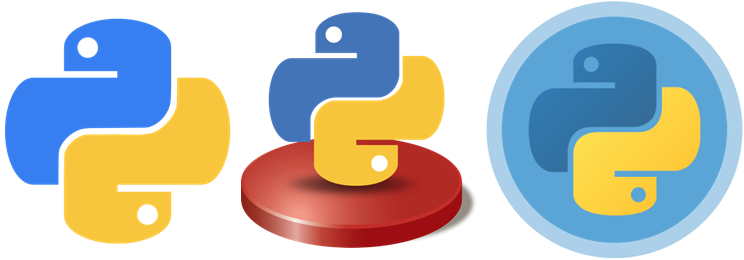
\includegraphics[width=12cm]{Python01.png} \\
       % {\tiny \sf Fonte: O autor deste trabalho }
    %\end{center}
   %\end{figure}

%Algumas figuras s\~{a}o criadas o elaboradas pelo mesmo autor, neste caso, deve-se escrever como fonte "O autor", "Os autores", etc. Figuras que incluam imagens de outras fontes deve-se especificar claramente, indicando o link o referencia correspondente, por exemplo, uma imagem que aparece em \cite[p. 93]{Sprankle2012}, \'{e} mostrada na Fig.\ref{afp} e a fonte deve ser indicada na parte inferior da figura.
   \begin{figure}[H]
    \begin{center}
        \caption{Algoritmo, Diagrama de fluxo, e Pseudo-código} \label{afp}
        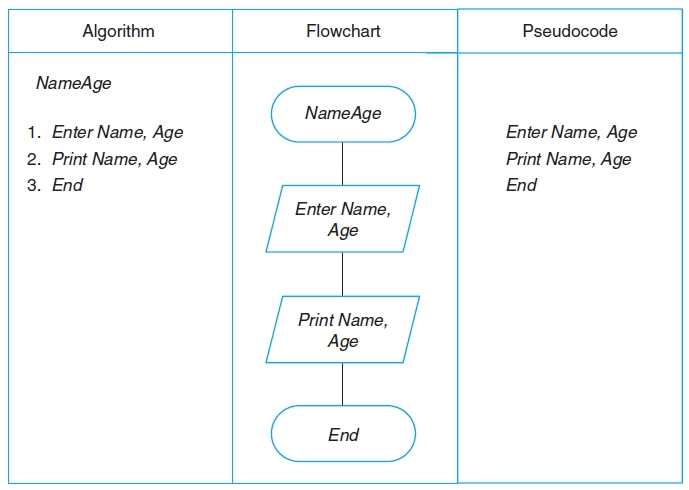
\includegraphics[width=10cm]{afp.jpg} \\
        {\tiny \sf Fonte: \cite[p. 93]{Sprankle2012} }
    \end{center}
   \end{figure}

   \section{Áreas de Aplicação da Linguagem}
   O Python está entre as linguagens de programação mais utilizadas no mundo, é utilizado por usuários individuais, mas sua aplicação se estende para empresas reais, como IBM, Seagate e Hewlett-Packard, que utilizam o Python para testes de hardware. O Yahoo! e Google usam a linguagem em serviços de Internet. Já a empresa Industrial Light and Magic e outras empresas de filmes utilizam o Python na produção de animações. Entre todas as aplicações para o Python atualmente, o ponto em comum é que a linguagem é usada em todo o espectro, em questão de domínios de aplicação.

        \subsection{Big Data}
        Python fornece um grande número de bibliotecas para trabalhar em Big Data. Você também pode trabalhar – em termos de desenvolvimento de código – usando Python para Big Data muito mais rápido do que qualquer outra linguagem de programação. Esses dois aspectos estão permitindo que desenvolvedores em todo o mundo adotem o Python como a linguagem de escolha para projetos de Big Data. 
        
        Para obter um conhecimento aprofundado sobre o Python juntamente com seus vários aplicativos, você pode se inscrever para o treinamento on-line ao vivo do Python com suporte 24 horas por dia, 7 dias por semana e acesso vitalício.
        
        É extremamente fácil lidar com qualquer tipo de dados em python. Vamos estabelecer isso com um exemplo simples. Você pode ver no instantâneo abaixo que o tipo de dados de 'a' é string e o tipo de dados de 'b' é inteiro. A boa notícia é que você não precisa se preocupar em lidar com o tipo de dados. Python já cuidou disso.

        \subsection{Orientação a objetos}
        A linguagem de programação Python é considerada orientada a objeto porque os valores são
        sempre armazenados em objetos. Em linguagens de programação diferentes de Python, os valores
        de certos tipos não são armazenados em entidades abstratas, como objetos, mas explicitamente na
        memória. O termo classe é usado para se referir aos tipos cujos valores são armazenados em
        objetos. Como cada valor em Python é armazenado em um objeto, cada tipo Python é uma classe. 
        
        Essa técnica de manipular dados, onde os dados são armazenados em objetos e os métodos são invocados sobre objetos, é chamada programação
        orientada a objeto (POO). A POO é uma técnica poderosa para organização e desenvolvimento
        de código. 

        \subsection{Outras} 